\section{An Overview of Machine Learning}
\label{sec:prelim-ml}
% Algorithmic review of classical ML, mined from thesis.tex's PRELIMINARIES
% (definitions, paradigms, figures) and condensed. Restructured on 20 Sep
% 2026 so that the section reviews *algorithms* -- ERM, the supervised and
% unsupervised methods, neural networks, learning on graphs -- rather than a
% survey of contemporary models. The kernel-methods and graph-learning
% material is new and is here because Chapter 4 depends on it.
This section reviews classical machine learning at the level of its
algorithms, to fix the vocabulary that the walk-based models of
Chapter~\ref{ch:methodology} are expressed in. It begins with the definition
of the learning problem and the paradigms into which it is divided, reviews
the supervised and unsupervised algorithms that the quantum models later
replace or extend --- with particular attention to kernel methods, on which
Application~II rests --- summarises neural networks and deep learning, and
closes with learning on graphs, which is the setting that unifies the
applications of this thesis. Two complete classical implementations follow,
whose structure the quantum implementations reproduce.

\subsection{Machine Learning as a Tool in Computer Science}
Machine learning is the study of programs whose behaviour on a task improves
with data rather than being fixed in advance. The definition usually credited
to Samuel~\cite{Samuel_1959}, who introduced the term, is informal.
\begin{definition}
The field of study that gives computers the ability to learn without being
explicitly programmed.
\end{definition}
Mitchell's definition~\cite{learning1997tom} is the operational one.
\begin{definition}
A computer program is said to learn from experience $E$ with respect to some
class of tasks $T$ and performance measure $P$ if its performance at $T$, as
measured by $P$, improves with experience $E$.
\end{definition}
The techniques have changed considerably since either definition was
written~\cite{alpaydin2021machine, ElNaqa2015}; the definitions themselves
have not needed to.

For the supervised case, which is the one Chapter~\ref{ch:methodology}
addresses, Mitchell's definition has a standard formalisation. The experience
is a training set $\{(x_i, y_i)\}_{i=1}^{m}$ of inputs $x_i \in \mathcal{X}$
and labels $y_i \in \mathcal{Y}$, drawn independently from an unknown
distribution $\mathcal{D}$; the task is to predict $y$ from $x$; and the
performance measure is the expected loss, or \emph{risk},
\begin{equation}
	R(h) = \mathbb{E}_{(x, y) \sim \mathcal{D}} \bigl[ \mathcal{L}(h(x), y) \bigr],
\end{equation}
of a hypothesis $h : \mathcal{X} \to \mathcal{Y}$ under a loss function
$\mathcal{L}$. Since $\mathcal{D}$ is unknown, a learning algorithm chooses
$h$ from a hypothesis class $\mathcal{H}$ by \emph{empirical risk
minimisation},
\begin{equation}
	\hat{h} = \arg\min_{h \in \mathcal{H}} \frac{1}{m} \sum_{i=1}^{m} \mathcal{L}(h(x_i), y_i) + \Omega(h),
	\label{eq:erm}
\end{equation}
where the regulariser $\Omega$ penalises complexity so that $\hat{h}$
generalises to unseen data rather than memorising the training set. Every
supervised algorithm below is an instance of~\eqref{eq:erm} distinguished by
its choice of $\mathcal{H}$, $\mathcal{L}$, $\Omega$ and the optimiser used
to solve it; the quantum models of Chapter~\ref{ch:methodology} change
$\mathcal{H}$ and leave the rest of the framework intact. The gap between
the empirical risk and $R(\hat{h})$ is the generalisation error, it is
estimated on data held out from training, and its control --- through
$\Omega$, through the size of $\mathcal{H}$, and through the amount of data
--- is the central practical problem of the field.

\subsection{Types of Machine Learning}
Introductory taxonomies present supervised, unsupervised and reinforcement
learning as mutually exclusive, which is a pedagogical simplification. The
paradigms are distinguished by the nature of the training signal and by what
data is available, and they overlap: reinforcement learning agents use
supervised losses for value prediction, and self-supervised learning is a
branch of unsupervised learning that manufactures its own labels.
Figure~\ref{fig:ml_paradigms} shows the relationships.

\begin{figure}[htbp]
\centering
\resizebox{0.85\textwidth}{!}{
	\begin{tikzpicture}[node distance=2.2cm, every node/.style={rectangle, draw, rounded corners, minimum width=2.8cm, minimum height=0.9cm, align=center, font=\small}, thick]
	\node (sup) {Supervised Learning};
	\node (uns) [right=of sup] {Unsupervised Learning};
	\node (ssl) [below=of uns] {Self-Supervised Learning};
	\node (semi) [below=of sup] {Semi-Supervised Learning};
	\node (rl) [below=of semi, xshift=1.4cm] {Reinforcement Learning};

	\draw[->, >=stealth] (ssl) -- node[above, sloped, draw=none, font=\footnotesize] {subset of} (uns);
	\draw[<->, >=stealth] (semi) -- node[above, sloped, draw=none, font=\footnotesize] {leverages} (sup);
	\draw[<->, >=stealth] (semi) -- node[above, sloped, draw=none, font=\footnotesize] {leverages} (uns);
	\draw[->, >=stealth, dashed] (rl.west) -- ++(-0.6,0) |- (sup.south);
	\draw[->, >=stealth, dashed] (rl.west) -- ++(-0.6,0) |- (uns.south);
	\node at (rl.west) [left=0.8cm, draw=none, font=\footnotesize] {may use either};
	\end{tikzpicture}
}
\caption{Conceptual relationships between the major machine-learning paradigms. Solid lines denote strong dependencies; dashed lines indicate optional methodological borrowing.}%
\label{fig:ml_paradigms}
\end{figure}

\subsubsection{Supervised Learning}
The model learns a mapping from inputs to labels from explicitly paired
examples by minimising~\eqref{eq:erm}. Representative algorithms are the
linear and logistic models, support vector machines, gradient-boosted trees
and neural networks reviewed below. Supervised learning is data-hungry and
assumes the training distribution is representative of the test distribution;
it is brittle under distribution shift and label noise, and acquiring labels
at scale is usually the practical bottleneck. Both applications of
Chapter~\ref{ch:methodology} are supervised classification.

\subsubsection{Unsupervised Learning}
The model operates on unlabelled data and seeks intrinsic structure --- a
clustering, a low-dimensional representation, a density. Representative
algorithms are $k$-means, principal component analysis and spectral
clustering, reviewed in Section~\ref{sec:ml-unsupervised}. With no ground
truth, evaluation is task-dependent, and different initialisations can yield
different results; the methods find statistical structure that need not be
semantically meaningful.

\subsubsection{Self-Supervised Learning}
Self-supervised learning generates its own supervisory signal from the input
by defining a pretext task --- predicting masked tokens or patches, or
learning representations invariant under augmentations --- and transfers the
resulting representation to downstream tasks. Masked language modelling and
contrastive methods are the representative algorithms. The quality of the
representation is sensitive to the pretext task, and a poorly chosen one
learns shortcuts that do not transfer. The random-walk embeddings of
Section~\ref{sec:ml-graphs} are self-supervised in exactly this sense.

\subsubsection{Reinforcement Learning}
Reinforcement learning does not start from a static dataset. An agent
interacts sequentially with an environment, receives a scalar reward, and
learns a policy from states to actions that maximises cumulative reward,
balancing exploration against exploitation; value-based methods such as deep
$Q$-networks and policy-gradient methods such as proximal policy optimisation
are representative. It is sample-inefficient, sensitive to reward design, and
its convergence guarantees are weaker than in the supervised setting. It is
not used in this thesis and is noted for completeness, though it has been
applied to the design of quantum-machine-learning architectures~\cite{Rapp_2024}.

\subsubsection{Semi-Supervised Learning}
Semi-supervised learning combines a small labelled set with a large
unlabelled one, on the assumption that the unlabelled data shapes the decision
boundary --- through consistency regularisation or pseudo-labelling. It relies
on the cluster and manifold assumptions, and when these fail the unlabelled
data can degrade performance. Node classification on a partially labelled
graph, the task of Section~\ref{sec:ml-graphs}, is the canonical
semi-supervised problem.

\subsection{Supervised Algorithms}
\label{sec:ml-supervised}
\subsubsection{Linear Models and Gradient Descent}
The simplest hypothesis class is linear, $h_w(x) = w^\top x + b$, and with
the squared loss equation~\eqref{eq:erm} is least-squares regression, solved
in closed form. For binary classification, $y \in \{-1, +1\}$, logistic
regression models $\Pr(y = 1 \mid x) = \sigma(w^\top x + b)$ with
$\sigma(z) = (1 + e^{-z})^{-1}$ and minimises the cross-entropy loss, which
has no closed form and is minimised by gradient descent,
$w \leftarrow w - \eta \nabla_w \hat{R}(w)$, or by its stochastic variant
using a mini-batch of examples per step. Stochastic gradient descent and its
adaptive-step descendants are the optimisers of every neural network in
Section~\ref{sec:ml-nn} and of every variational quantum model in
Chapter~\ref{ch:methodology}; the only thing that changes in the quantum
case is how the gradient is evaluated.

\subsubsection{Nearest Neighbours and Trees}
The $k$-nearest-neighbour classifier assigns to $x$ the majority label among
the $k$ training points closest to it under a chosen metric; it has no
training phase, its cost is entirely at prediction time, and it depends
entirely on the metric --- which is the sense in which it is the simplest
similarity-based method, a family that Application~II belongs to. Decision
trees partition $\mathcal{X}$ recursively by axis-aligned thresholds chosen
to maximise a purity criterion, and gradient boosting fits a sequence of
shallow trees, each to the residual of the ensemble so far; boosted trees
remain the strongest general-purpose method on tabular data and are the
classical baseline one should expect a quantum model on such data to be
measured against~\cite{Bowles_2024}.

\subsubsection{Kernel Methods and Support Vector Machines}
\label{sec:ml-kernels}
The support vector machine~\cite{Valkenborg_2023, Awad_2015} chooses, among
the linear classifiers separating two classes, the one with the largest
margin. For linearly separable data with $y_i \in \{-1, +1\}$ this is
\begin{equation}
	\min_{w, b} \tfrac{1}{2} \|w\|^2 \quad \text{subject to} \quad y_i (w^\top x_i + b) \ge 1 \ \ \forall i,
\end{equation}
and for data that is not separable a slack term $C \sum_i \xi_i$ is added
to the objective with the constraints relaxed to
$y_i(w^\top x_i + b) \ge 1 - \xi_i$. The dual problem is a quadratic programme
in Lagrange multipliers $\alpha_i \ge 0$,
\begin{equation}
	\max_{\alpha} \sum_i \alpha_i - \frac{1}{2} \sum_{i, j} \alpha_i \alpha_j y_i y_j\, \langle x_i, x_j \rangle
	\quad \text{subject to} \quad \sum_i \alpha_i y_i = 0, \quad 0 \le \alpha_i \le C,
	\label{eq:svmdual}
\end{equation}
whose solution gives $w = \sum_i \alpha_i y_i x_i$ and the classifier
$h(x) = \operatorname{sgn}\bigl(\sum_i \alpha_i y_i \langle x_i, x \rangle + b\bigr)$.
The training points with $\alpha_i > 0$ are the support vectors.

Equation~\eqref{eq:svmdual} depends on the data only through inner products,
and that is the observation on which kernel methods rest~\cite{Hofmann_2008}.
If the inputs are first mapped into a feature space by
$\Phi : \mathcal{X} \to \mathcal{F}$, the inner products become
$k(x, x') = \langle \Phi(x), \Phi(x') \rangle_{\mathcal{F}}$, and the whole
algorithm --- training and prediction --- can be run knowing only the
\emph{kernel function} $k$, never $\Phi$ itself. The $m \times m$ Gram matrix
$K_{ij} = k(x_i, x_j)$ is all the training algorithm consumes. A function $k$
is a valid kernel exactly when every Gram matrix it produces is symmetric
positive semi-definite, in which case $\Phi$ exists (possibly into an
infinite-dimensional space) by Mercer's theorem. The Gaussian kernel
$k(x, x') = \exp(-\gamma \|x - x'\|^2)$ and polynomial kernels
$(\langle x, x' \rangle + c)^p$ are the standard choices; a kernel can also
be defined directly on structured objects such as strings or graphs, without
a vector representation, which is what makes the method applicable to graph
learning. The quantum kernel methods of Application~II are precisely this
algorithm with $\Phi$ realised by a quantum circuit and $k$ estimated from
measurements, and Chapter~\ref{ch:methodology} states what that changes and
what it leaves untouched.

\subsection{Unsupervised Algorithms}
\label{sec:ml-unsupervised}
Three unsupervised algorithms are needed later, each because a quantum
analogue of it appears in the walk literature reviewed in
Section~\ref{ch:litreview}.

\emph{$k$-means} partitions $m$ points into $k$ clusters by alternately
assigning each point to the nearest of $k$ centroids and moving each centroid
to the mean of its assigned points, until the assignments stop changing; it
minimises the within-cluster sum of squares, converges to a local optimum
that depends on the initialisation, and assumes clusters that are convex in
the chosen metric. \emph{Principal component analysis} projects the data onto
the leading eigenvectors of its covariance matrix, giving the linear
projection of a chosen dimension that preserves the most variance; it is the
standard dimensionality reduction and the standard preprocessing step before
a classifier, including the ones in Chapter~\ref{ch:methodology}.
\emph{Spectral clustering} builds a similarity graph on the data, computes
the leading eigenvectors of its Laplacian, and runs $k$-means in the
resulting coordinates; it finds clusters that $k$-means cannot, at the cost
of an eigendecomposition, and its behaviour on sparse graphs is delicate
enough to have a literature of its own~\cite{Krzakala_2013}. Spectral
clustering is the algorithm in which the graph Laplacian of
Section~\ref{sec:ctqw} first appears in machine learning, and the
walk-based community-detection methods reviewed in Section~\ref{ch:litreview}
are its quantum descendants.

\subsection{Neural Networks and Deep Learning}
\label{sec:ml-nn}
An artificial neural network is a composition of layers, each an affine map
followed by an element-wise non-linearity,
\begin{equation}
	h(x) = f_L \circ \cdots \circ f_1 (x), \qquad f_\ell(z) = \sigma_\ell(W_\ell z + b_\ell),
	\label{eq:mlp}
\end{equation}
whose parameters $\{W_\ell, b_\ell\}$ are learned by minimising~\eqref{eq:erm}
with gradient descent; the gradient of the loss with respect to every
parameter is computed by \emph{backpropagation}, which is the chain rule
applied layer by layer from the output backwards, and the cost of one
gradient evaluation is a small constant times the cost of one forward pass.
Figure~\ref{fig: neural_network} shows the feed-forward structure. A network
with one sufficiently wide hidden layer can approximate any continuous
function on a compact set, so the hypothesis class is universal; what
determines success in practice is the architecture --- how $W_\ell$ is
constrained --- and the optimiser.

\begin{figure}[htbp]
	\centering
	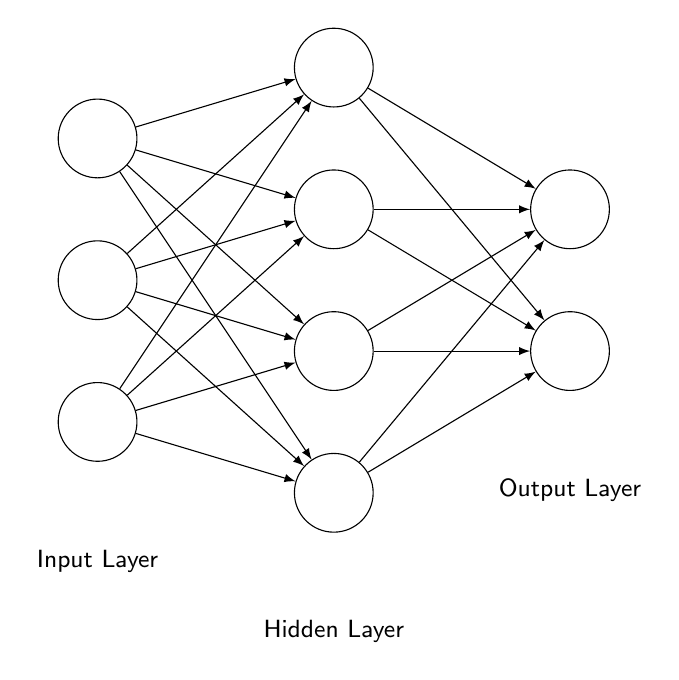
\begin{tikzpicture}[
		>=latex,
		neuron/.style={circle, draw, fill=white, minimum size=1cm, inner sep=0pt},
		layerlabel/.style={font=\sffamily\small, below=1.5cm}
	]
		\def\vdist{1.8}
		\foreach \i in {1,2,3} {
			\node[neuron] (I\i) at (0, {\vdist*(1-\i)}) {};
		}
		\node[layerlabel] (L1) at (0, {-2*\vdist}) {Input Layer};
		\foreach \i in {1,2,3,4} {
			\node[neuron] (H\i) at (3, {\vdist*(1.5-\i)}) {};
		}
		\node[layerlabel] (L2) at (3, {-2.5*\vdist}) {Hidden Layer};
		\foreach \i in {1,2} {
			\node[neuron] (O\i) at (6, {\vdist*(0.5-\i)}) {};
		}
		\node[layerlabel] (L3) at (6, {-1.5*\vdist}) {Output Layer};
		\foreach \i in {1,2,3} {
			\foreach \j in {1,2,3,4} {
				\draw[->] (I\i) -- (H\j);
			}
		}
		\foreach \i in {1,2,3,4} {
			\foreach \j in {1,2} {
				\draw[->] (H\i) -- (O\j);
			}
		}
	\end{tikzpicture}
	\caption{Structure of a simple feed-forward neural network}%
	\label{fig: neural_network}
\end{figure}

Deep learning is the regime in which $L$ is large and the layers are
structured. Convolutional networks constrain $W_\ell$ to be a convolution,
sharing weights across positions and giving translation equivariance, and
dominate image tasks; recurrent networks apply the same layer at each step of
a sequence, carrying a hidden state, and were the standard sequence model
until the transformer~\cite{NIPS2017_3f5ee243} replaced recurrence with
\emph{self-attention}, in which every position computes a weighted average of
every other position with weights learned from the data, and processes the
whole sequence in parallel. Autoencoders learn a compressed representation
by training an encoder--decoder pair to reconstruct their input, and are the
basis of generative models; generative adversarial networks and diffusion
models are the two dominant generative families. Graph neural networks
constrain the layer to aggregate over a vertex's neighbours, so that the
representation of a vertex after $L$ layers depends on its $L$-hop
neighbourhood~\cite{NIPS2017_5dd9db5e}; they are the deep-learning approach
to the graph problems of the next subsection, and the quantum-walk neural
networks reviewed in Section~\ref{ch:litreview} are their walk-based
counterparts. The parameterised quantum circuits of Application~I occupy the
place of~\eqref{eq:mlp}: the layers are unitaries, the parameters are gate
angles, and the loss is a measured expectation value; the optimiser and the
training loop are unchanged.

\subsection{Learning on Graphs}
\label{sec:ml-graphs}
The applications of this thesis are unified by the graph. A learning problem
is a graph problem when the input carries a relational structure --- the
edges of a network, the bonds of a molecule, the adjacency of pixels or
features --- that a vector representation discards. The three standard tasks
are \emph{node classification}, in which the vertices of one partially
labelled graph are to be labelled (the citation networks of Sen et
al.~\cite{Sen_2008} are the standard benchmarks, and the setting is
semi-supervised); \emph{link prediction}; and \emph{graph classification},
in which each example is a whole graph and the label is a property of it.

Classical algorithms attack these tasks in three ways, and all three have
walk-based quantum analogues in the literature of
Section~\ref{ch:litreview}. \emph{Node embedding} learns a vector for each
vertex such that the geometry of the vectors reflects the structure of the
graph; the dominant methods sample random walks from each vertex and train
the embedding, self-supervised, to predict a vertex's walk co-occurrences ---
DeepWalk~\cite{Perozzi_2014} with uniform walks, node2vec~\cite{Grover_2016}
with a biased second-order walk that interpolates between breadth-first and
depth-first exploration --- and the embeddings are then fed to any
supervised classifier~\cite{Xia_2020, doi:10.1137/20M1386062, Bozorgi_2024}.
The classical random walk is the feature extractor, which is exactly the
place the quantum walk can be substituted; that substitution is the
QWalkVec line of work reviewed in Section~\ref{sec:lr-dtqwqml}, and it is not
pursued in this thesis. \emph{Graph kernels} define $k(G, G')$ directly on graphs, most
often by comparing the distributions of walks or substructures the two
graphs contain, and hand the result to the support vector machine of
Section~\ref{sec:ml-kernels}; Application~II is the quantum version of this
idea, with the walk run coherently rather than sampled. \emph{Graph neural
networks} learn the aggregation end-to-end, and Application~I's walk-based
feature maps are one way of building the adjacency into a quantum
circuit's layers. The two applications are thus two entry points of the
walk into one problem, with the graph-classification experiments of
Section~\ref{sec:graphresults} as the case where the graph is itself the
datum, and it is in that sense that the problem statement of
Chapter~\ref{ch:intro} is framed around graph learning.

The two listings themselves are reproduced in Appendix~\ref{app:listings}:
a TensorFlow text classifier and a PyTorch image classifier, both
tutorial-level examples and neither a contribution of this thesis. They are
the template the quantum implementations of
Chapter~\ref{ch:methodology} follow, with the model definition replaced by a
circuit, and the library idioms they exhibit recur in the quantum libraries.


